\section{Problem statement}
To better understand the computational challenge before us, we begin by formulating the physical setup.
The force exerted on a body with mass $m_2$ at the point $\mathbf{x}_2$ by a body with mass $m_1$ located at $\mathbf{x}_1$ can be expressed by the relation
\begin{equation}\label{eq:law-of-uni-grav}
    \mathbf{F} = -G\frac{m_1m_2}{|\mathbf{x}_{21}|^3}\mathbf{x}_{21}
\end{equation}
where $G$ is the gravitational constant $6.674\times 10^{-11}\, \mathrm{m}^3 \,\mathrm{kg}^{-1}\,\mathrm{s}^{-2}$ and $\mathbf{x}_{21} = \mathbf{x}_2 - \mathbf{x}_1$.
Therefore, the evolution of a system of $N$ bodies is governed by $N$ equations
\begin{equation}\label{eq:pp-method}
    \ddot{\mathbf{x}}_i = -G\sum_{j\neq i} \frac{m_j}{|\mathbf{x}_{ij}|^3}\mathbf{x}_{ij}.
\end{equation}
for each $i = 1,\dots, N$.
Direct application of \autoref{eq:pp-method} is the basis of the so-called \textit{particle-particle} (PP) method.
The method is characterized by $O(N^2)$ time complexity (more precisely, it requires $(N-1)N/2$ operations if Newton's 3rd law is used in the computation).
This running time characteristic $T(N)$ (running time of one simulation iteration) can be directly observed by running an implementation of the method (see \autoref{fig:pp-method-scaling}).
\begin{figure}[htp]
    \centering
    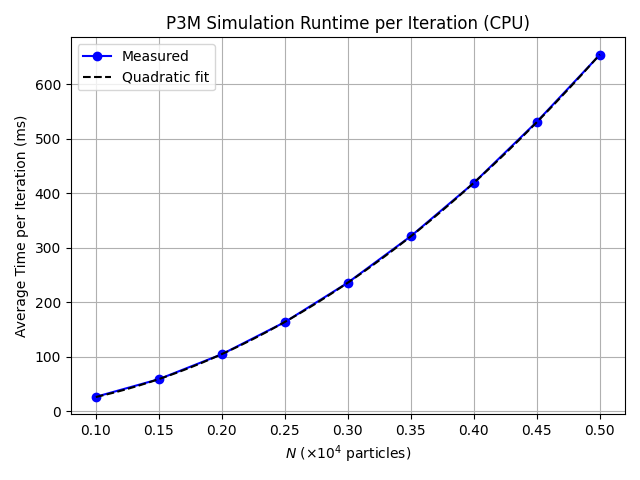
\includegraphics[scale=0.5]{chapters/introduction/img/pp_time.png}
    \caption{Scaling of the PP method.}
    \label{fig:pp-method-scaling}
\end{figure}
The exact form of $T(N)$ depends on the implementation details and the type of hardware used, but assuming that the code whose running time is shown in \autoref{fig:pp-method-scaling} is not tragically inefficient, we can draw some general conclusions regarding the applicability of the PP method.
Fitting a quadratic through the points shown in the figure reveals the following approximation: $T(1{,}000N) \approx 26.1N^2 + 0.32N$ [ms].
In a reasonable particle simulation, one often deals with tens of thousands of particles (if not more) and the simulation can span hundreds of iterations.
Thus, assuming sensible values of $N = 50{,}000$ and 200 iterations, we get the expected running time of $\approx 3.5$ hours!
This clearly shows that more efficient algorithms have to be put in place.
